% ============================================================
% 第五章 飞行控制系统配置与调试
% ============================================================

\chapter{飞行控制系统配置与调试}

\section{多旋翼飞行动力学分析}

\subsection{坐标系定义}

本文采用右手坐标系进行动力学建模。
地理坐标系（惯性系）以起飞点为原点，$x$ 轴指向正北，$y$ 轴指向正东，$z$ 轴竖直向下。
机体坐标系固连于飞行器，原点位于质心，$x_b$ 轴指向机头方向，
$y_b$ 轴指向机身右侧，$z_b$ 轴向下。
姿态角采用欧拉角表示：滚转角 $\phi$、俯仰角 $\theta$、偏航角 $\psi$。

\subsection{六自由度运动方程}

多旋翼飞行器作为刚体，其运动由平动方程与转动方程共同描述。

\textbf{平动方程}（在惯性系下）：

\begin{equation}
    m\ddot{\boldsymbol{p}} = m\boldsymbol{g} + \boldsymbol{R} \cdot \boldsymbol{F}_b
    \label{eq:translation}
\end{equation}

其中 $\boldsymbol{p}$ 为位置向量，$\boldsymbol{R}$ 为从机体系到惯性系的旋转矩阵，
$\boldsymbol{F}_b = [0,\,0,\,-T_{\text{total}}]^T$ 为机体系下的合力（升力沿 $z_b$ 负方向）。

\textbf{转动方程}（在机体系下）：

\begin{equation}
    \boldsymbol{I}\dot{\boldsymbol{\omega}} + \boldsymbol{\omega} \times (\boldsymbol{I}\boldsymbol{\omega}) = \boldsymbol{\tau}
    \label{eq:rotation}
\end{equation}

其中 $\boldsymbol{I}$ 为转动惯量矩阵，$\boldsymbol{\omega} = [p,\,q,\,r]^T$ 为机体角速度，
$\boldsymbol{\tau} = [\tau_\phi,\,\tau_\theta,\,\tau_\psi]^T$ 为控制力矩。

对于正方形四旋翼X型布局，控制分配矩阵将四个电机推力
$[T_1,\,T_2,\,T_3,\,T_4]^T$ 映射为升力与三轴力矩：

\begin{equation}
    \begin{bmatrix} T_{\text{total}} \\ \tau_\phi \\ \tau_\theta \\ \tau_\psi \end{bmatrix}
    =
    \begin{bmatrix}
        1 &  1 &  1 &  1 \\
        L & -L & -L &  L \\
        L &  L & -L & -L \\
        k & -k &  k & -k
    \end{bmatrix}
    \begin{bmatrix} T_1 \\ T_2 \\ T_3 \\ T_4 \end{bmatrix}
    \label{eq:allocation}
\end{equation}

其中 $L = 0.435$\,m 为旋翼到机体坐标轴的力臂，$k$ 为电机反扭矩系数。

\subsection{充气伞形结构对飞行动力学的影响}

本系统相较于标准多旋翼飞行器，在动力学层面存在两项显著差异。

\subsubsection{转动惯量显著偏大}

以旋翼平面几何中心为转动基准，对系统各主要部件的转动惯量进行估算，
结果如表~\ref{tab:inertia}所示。

\begin{table}[htbp]
    \centering
    \caption{各部件转动惯量估算（绕 $x/y$ 轴）}
    \label{tab:inertia}
    \begin{tabular}{lrrr}
        \toprule
        部件              & 质量 (g) & 等效力臂 (mm) & $I_{xx}$ (kg$\cdot$m$^2$) \\
        \midrule
        旋翼单元 $\times 4$  & 492  & 435  & 0.093 \\
        PLA节点结构件        & 600  & 350  & 0.065 \\
        气柱骨架             & 150  & 均布  & 0.019 \\
        TPU伞面             & 150  & 均布  & 0.019 \\
        中心件（飞控等）      &  76  & $\approx 0$ & $\approx 0$ \\
        \midrule
        \textbf{合计}        & —    & —    & \textbf{0.196} \\
        \bottomrule
    \end{tabular}
\end{table}

本系统 $I_{xx} = I_{yy} \approx 0.196$\,kg$\cdot$m$^2$，
$I_{zz} \approx 0.393$\,kg$\cdot$m$^2$。
相比典型450\,mm轴距四旋翼（$I_{xx} \approx 0.012$\,kg$\cdot$m$^2$），
本系统转动惯量\textbf{约为标准四旋翼的16倍}，
主要来源于1230\,mm超大轴距与大面积骨架的质量分布。

转动惯量大意味着：相同控制力矩下角加速度更小，姿态响应较慢；
但同时在低速悬停时对小扰动的角加速度响应更迟钝，
飞行器表现出更好的姿态自然稳定性。
在PID参数整定时，大转动惯量要求\textbf{显著降低比例增益P}，
否则控制力矩相对于惯量过强，易引发姿态震荡。

\subsubsection{重心略高于旋翼平面}

由第四章计算，整机质心位于旋翼平面上方约6\,mm处。
该偏高幅度相对于1230\,mm旋翼轴距仅约0.5\%，
对飞行稳定性影响极小，在正常PID控制范围内可完全补偿，
无需进行配重调整或特殊控制策略设计。


\section{Pixhawk 6C嵌入式飞控系统}

\subsection{硬件架构}

本系统选用 \textbf{Pixhawk 6C} 开源飞控硬件平台。
Pixhawk 6C搭载STM32H753主处理器（480\,MHz）与STM32F100协处理器，
集成三轴加速度计与陀螺仪（ICM-42688-P）、
气压计（MS5611）、磁罗盘接口等传感器，
运行 \textbf{NuttX实时操作系统}与 \textbf{PX4飞控固件}。
主要硬件参数如表~\ref{tab:pixhawk_spec}所示。

\begin{table}[htbp]
    \centering
    \caption{Pixhawk 6C 主要硬件参数}
    \label{tab:pixhawk_spec}
    \begin{tabular}{ll}
        \toprule
        参数           & 规格 \\
        \midrule
        主处理器        & STM32H753（480\,MHz，2\,MB Flash） \\
        加速度计/陀螺仪 & ICM-42688-P \\
        气压计          & MS5611 \\
        工作电压        & 4.75$\sim$5.25\,V \\
        自重            & 约38\,g \\
        PWM输出         & 8路 \\
        通信接口        & UART $\times$6，I$^2$C $\times$2，SPI $\times$3 \\
        \bottomrule
    \end{tabular}
\end{table}

\subsection{PX4控制回路架构}

PX4固件实现了完整的多旋翼飞行控制回路，采用\textbf{内外环级联控制}结构：

\begin{itemize}
    \item \textbf{姿态控制回路（内环）}：以IMU测量的角速度与姿态角为反馈，
          通过PID控制器输出控制力矩指令，再经控制分配矩阵转换为各电机PWM指令。
          姿态回路运行频率约250$\sim$1000\,Hz。
    \item \textbf{位置控制回路（外环）}：以GPS/气压计测量的位置与速度为反馈，
          输出期望姿态角指令给姿态回路。位置回路运行频率约50\,Hz。
\end{itemize}

本系统在验证阶段主要使用\textbf{姿态稳定模式（Stabilize）}
与\textbf{定高模式（Altitude Hold）}，
通过乐迪AT9S Pro遥控器进行手动控制，不涉及全自主飞行。

% ----------------------------------------------------------
% [图片占位 Fig.5.1] ★推荐制作★
% 内容：PX4双环控制回路框图
%   外环（位置控制）→ 期望姿态角 → 内环（姿态控制）→ 电机PWM → 飞行器
%   可参考PX4官方文档的控制架构图，手绘或用draw.io简化绘制
% \begin{figure}[htbp]
%     \centering
%     \includegraphics[width=0.80\textwidth]{figures/fig5_1_px4_control_loop.png}
%     \caption{PX4双环级联控制回路架构}
%     \label{fig:px4_loop}
% \end{figure}
% ----------------------------------------------------------

\subsection{传感器配置与校准}

飞控系统集成以下传感器，均通过QGroundControl（QGC）地面站完成校准：

\begin{itemize}
    \item \textbf{IMU}：六点加速度计校准，消除零偏与比例误差；陀螺仪上电自动校准；
    \item \textbf{磁罗盘}：椭球拟合旋转校准，消除硬铁/软铁干扰；
    \item \textbf{气压计}：自动温度补偿，用于定高模式高度保持；
    \item \textbf{遥控器}：通道映射与摇杆行程校准，油门曲线线性化设置。
\end{itemize}

由于本系统骨架为气柱薄膜材料（无铁磁性），对磁罗盘的干扰极小，
磁罗盘校准结果良好。四个ESC通过物理隔离（远离飞控安装位）
有效抑制无刷电机工作时的电磁干扰。


\section{针对充气伞形结构的PID参数整定}

\subsection{整定难点分析}

本系统在PID参数整定方面面临以下有别于标准多旋翼的特殊挑战：

\begin{itemize}
    \item \textbf{大转动惯量导致的响应迟滞}：
          如5.1节分析，本系统转动惯量约为同质量标准四旋翼的16倍。
          若照搬标准四旋翼PID参数，比例项P过大会导致控制力矩远超实际需求，
          引发姿态过冲甚至持续震荡；初始整定时须显著降低P增益。

    \item \textbf{伞面气动阻尼的影响}：
          充气伞面的大面积对空气运动产生显著的气动阻尼，
          使系统在横向扰动下具有较大的自然衰减效果，
          有利于减少超调，但可能造成姿态响应不灵敏，
          需适当补偿微分项D。

    \item \textbf{悬停油门预设}：
          本系统悬停油门约26\%$\sim$30\%，
          远低于PX4默认的50\%悬停油门预设，
          需在飞行前通过参数 \texttt{MPC\_THR\_HOVER} 进行修正，
          否则飞控在切换定高模式时会产生较大的高度跳变。
\end{itemize}

\subsection{初始PID参数设置}

鉴于本系统大转动惯量特性，初始参数在PX4默认值基础上进行调整，
如表~\ref{tab:pid_params}所示。

\begin{table}[htbp]
    \centering
    \caption{PID参数初始设定值（相对PX4默认值）}
    \label{tab:pid_params}
    \begin{tabular}{lrrl}
        \toprule
        参数名称             & PX4默认值 & 初始设定值 & 调整依据 \\
        \midrule
        \texttt{MC\_ROLLRATE\_P}   & 0.150 & 0.050 & 大转动惯量，P降至默认值1/3 \\
        \texttt{MC\_ROLLRATE\_I}   & 0.100 & 0.050 & 保留I项消除稳态误差 \\
        \texttt{MC\_ROLLRATE\_D}   & 0.003 & 0.008 & D适当增大补偿气动阻尼 \\
        \texttt{MC\_PITCHRATE\_P}  & 0.150 & 0.050 & 同Roll轴 \\
        \texttt{MC\_PITCHRATE\_I}  & 0.100 & 0.050 & 同Roll轴 \\
        \texttt{MC\_PITCHRATE\_D}  & 0.003 & 0.008 & 同Roll轴 \\
        \texttt{MC\_YAWRATE\_P}    & 0.200 & 0.080 & 偏航惯量更大，P进一步降低 \\
        \texttt{MC\_YAWRATE\_I}    & 0.100 & 0.040 & — \\
        \texttt{MPC\_THR\_HOVER}   & 0.500 & 0.280 & 悬停油门约26\%$\sim$30\% \\
        \bottomrule
    \end{tabular}
\end{table}

\subsection{整定流程}

参数整定依照以下步骤进行，全程使用QGC地面站实时监控飞行状态与日志：

\begin{description}
    \item[第一步：机型配置]
        在QGC中选择机型为"Generic Quadrotor X"，
        按PX4标准X型四旋翼顺序连接电机：
        1号（右前，逆时针）、2号（左后，逆时针）、
        3号（左前，顺时针）、4号（右后，顺时针）。

    \item[第二步：传感器校准]
        依次完成加速度计六点校准、磁罗盘旋转校准、
        遥控器通道校准与油门曲线线性化设置。

    \item[第三步：参数预设]
        按表~\ref{tab:pid_params}输入初始PID参数，
        同时设置 \texttt{MPC\_THR\_HOVER = 0.28}，
        \texttt{MOT\_SPIN\_MIN = 0.05}（最低电机转速，防止低油门停转）。

    \item[第四步：绑绳悬停测试]
        用四根软绳（约1\,m长）从四个方向固定飞行器，
        推油门至悬停点，观察飞行器姿态稳定性与震荡情况。
        若出现明显的Roll/Pitch震荡，继续降低对应轴的P增益；
        若响应过于迟钝，适当增大D增益。

    \item[第五步：自由悬停精调]
        解除绑绳，在空旷场地进行自由悬停测试，
        根据实际姿态响应逐步微调P、I、D参数至稳定悬停状态。
        调整原则：P决定响应速度，I消除稳态漂移，D抑制过冲。
\end{description}

% ----------------------------------------------------------
% [图片占位 Fig.5.2] ★推荐制作★
% 内容：QGC地面站参数配置界面截图
%   截图内容：Parameters页面，显示MC_ROLLRATE_P等参数输入框
%   或：飞行日志中Roll/Pitch角度曲线，显示调参前后对比
%   用QGC软件截图即可，无需额外绘制
% \begin{figure}[htbp]
%     \centering
%     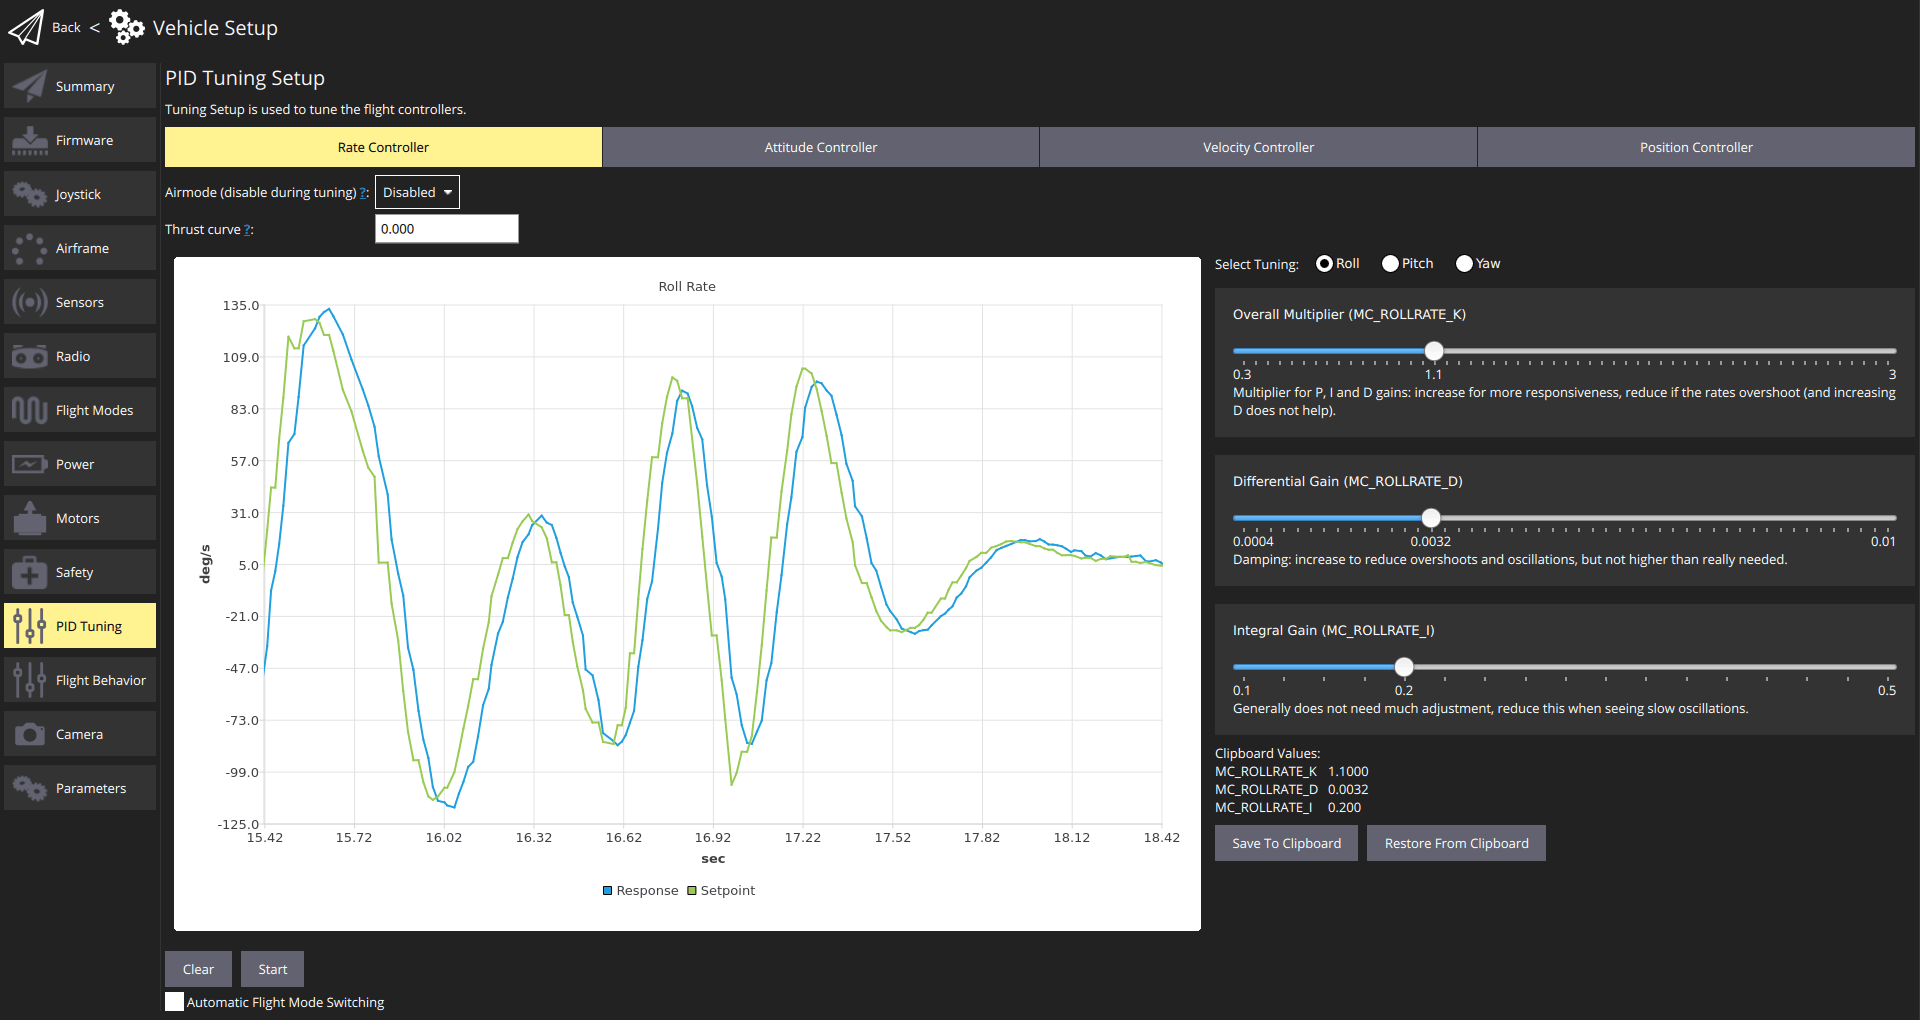
\includegraphics[width=0.75\textwidth]{figures/fig5_2_qgc_params.png}
%     \caption{QGroundControl地面站PID参数配置界面}
%     \label{fig:qgc_params}
% \end{figure}
% ----------------------------------------------------------


\section{通信链路配置}

\subsection{遥控链路}

本系统使用\textbf{乐迪AT9S Pro}遥控器（9通道，2.4\,GHz FHSS跳频扩频技术），
配套R9DS接收机通过SBUS协议与Pixhawk 6C连接。
控制信号链路如下：

\begin{center}
AT9S Pro遥控器
$\xrightarrow{\text{2.4\,GHz FHSS}}$
R9DS接收机
$\xrightarrow{\text{SBUS}}$
Pixhawk 6C
$\xrightarrow{\text{PWM/DSHOT}}$
ESC $\times 4$
$\rightarrow$
电机 $\times 4$
\end{center}

遥控器通道分配如下：
通道1（副翼/Roll）、通道2（升降/Pitch）、
通道3（油门/Throttle）、通道4（方向/Yaw）、
通道5（飞行模式切换）、通道6（紧急锁定/Kill Switch）。

\subsection{失控保护配置}

AT9S Pro支持失控保护（Failsafe）功能：
当遥控信号持续丢失超过0.5\,s时，
飞控自动执行预设的失控保护动作。
结合本系统最大飞行高度不超过2\,m的工作约束，
失控保护动作设置为\textbf{原地降落（Land）}模式，
确保在任何情况下飞行器均能安全落地，不会对周围人员造成安全威胁。


\section{本章小结}

本章完成了飞行雨伞系统飞行控制系统的配置与调试方案设计。
通过建立多旋翼六自由度动力学模型，分析了充气伞形结构对飞行动力学的两项特殊影响：
转动惯量约为标准四旋翼的16倍（$I_{xx} \approx 0.196$\,kg$\cdot$m$^2$），
以及质心偏高约6\,mm。
基于Pixhawk 6C飞控平台与PX4固件，完成了传感器校准、
电机接线配置与飞行模式设置。
针对大转动惯量特性，制定了系统性的PID参数初始整定策略，
将Roll/Pitch比例增益降至PX4默认值的1/3，
并提出了绑绳悬停→自由悬停的渐进式调试流程，
为飞行验证阶段提供了完整的调试方案。